% ===
%
% Official LaTeX seminar report template of the
% Chair for AI Methodology (AIM)
% RWTH Aachen University, Aachen, Germany
%
% Author: Jakob Bossek (bossek@aim.rwth-aachen.de)
%
% AIM website: https://aim.rwth-aachen.de/
%
% ===

% The 'review' option activates line numbering
\documentclass[review]{AIM_report}

% includes/preamble.tex is the right place to add new packages etc.
% tables
\RequirePackage{booktabs}
\RequirePackage{colortbl}
\RequirePackage{multicol}
\RequirePackage{multirow}
\RequirePackage{xspace}
\RequirePackage[final]{pdfpages}

% \smiley{} and \frowney{}
\RequirePackage{wasysym}

% quotation
\RequirePackage{csquotes}

% side-by-side sub-figures
\RequirePackage{subcaption}


% import commenting macros
\input{includes/macros/commenting}

% metadata
\title{Adversarial Attacks (AA)}
\subtitle{Robust Deep Learning (Seminar)}
\author{Bjarne Thal (446558) and Marius Wrobel (456734)}

\institute{RWTH Aachen University, Germany\\
\email{$\{$bjarne.thal, marius.wrobel$\}$@rwth-aachen.de}}  

% source file(s) with bibliography entries
\addbibresource{bib.bib}
\usepackage{graphicx}
\begin{document}

\maketitle
\section{Introduction}
\label{sec:intro}

Over the past decade, deep neural networks have become the dominant approach for a broad range of perception tasks, from image classification and speech recognition to natural language understanding; in many cases matching or surpassing human performance~\cite{lecun2015deep, he2015delving}. Due to their strength, such models are increasingly deployed in critical settings, such as autonomous driving~\cite{grigorescu2020survey}  or biometric identification~\cite{schroff2015facenet}.

This success, however, is built upon a surprisingly fragile foundation. In 2013, Szegedy et al.\ \cite{szegedy2013intriguing} showed that state-of-the-art classifiers can be fooled by \textit{adversarial examples}: inputs altered by a perturbation so small that it is imperceptible to a human, yet enough to make the model produce a confident but incorrect prediction. Such examples are neither rare accidents nor isolated mistakes of a single model: the same perturbed input frequently fools different architectures trained on different data, furthermore the vulnerability appears across all kinds of machine learners~\cite{goodfellow2014explaining, biggio2018wild}. This portability across models---known as \textit{transferability}---is one of the defining characteristics of adversarial examples and a large part of their appeal as an object of study, as it even enables attacks against models the adversary cannot directly inspect.

This report serves as a broad introduction to the topic of adversarial attacks. In our examination of specific attack methods, we thus concentrate on the classical setting of evasion and poisoning attacks against image classifiers, surveying the ideas and methods that have shaped the research area. We focus on image classification throughout, both because the bulk of the research area centres on this setting and because its inherently visual nature of such tasks mean easily interpretable illustrations. We do focus on evasion attacks as in the kick-off lecture and include the poisoning attacks as another interesting approach. 

The rest of the report is organised as follows. Section~\ref{sec:attacks} defines adversarial examples, introduces a taxonomy of adversarial attacks, and reviews the most influential evasion and poisoning attacks. Section~\ref{sec:discussion} then contains our discussion: the pertinence of adversarial attacks in the real and physical world, the competing attempts to explain why adversarial examples exist in the first place, and a reflection on what makes the phenomenon a worthwhile object of study.




\section{Adversarial Attacks}
\label{sec:attacks}
\subsection{Definition}
\textit{Adversarial attacks} can be described as inputting \textit{adversarial examples} into a machine learning system~\cite{brendel2017decision}. These two terms were introduced by Szegedy et al.~\cite{szegedy2013intriguing} and have since been used in different variations; here, we use the following definition:

\begin{figure}
    \centering
    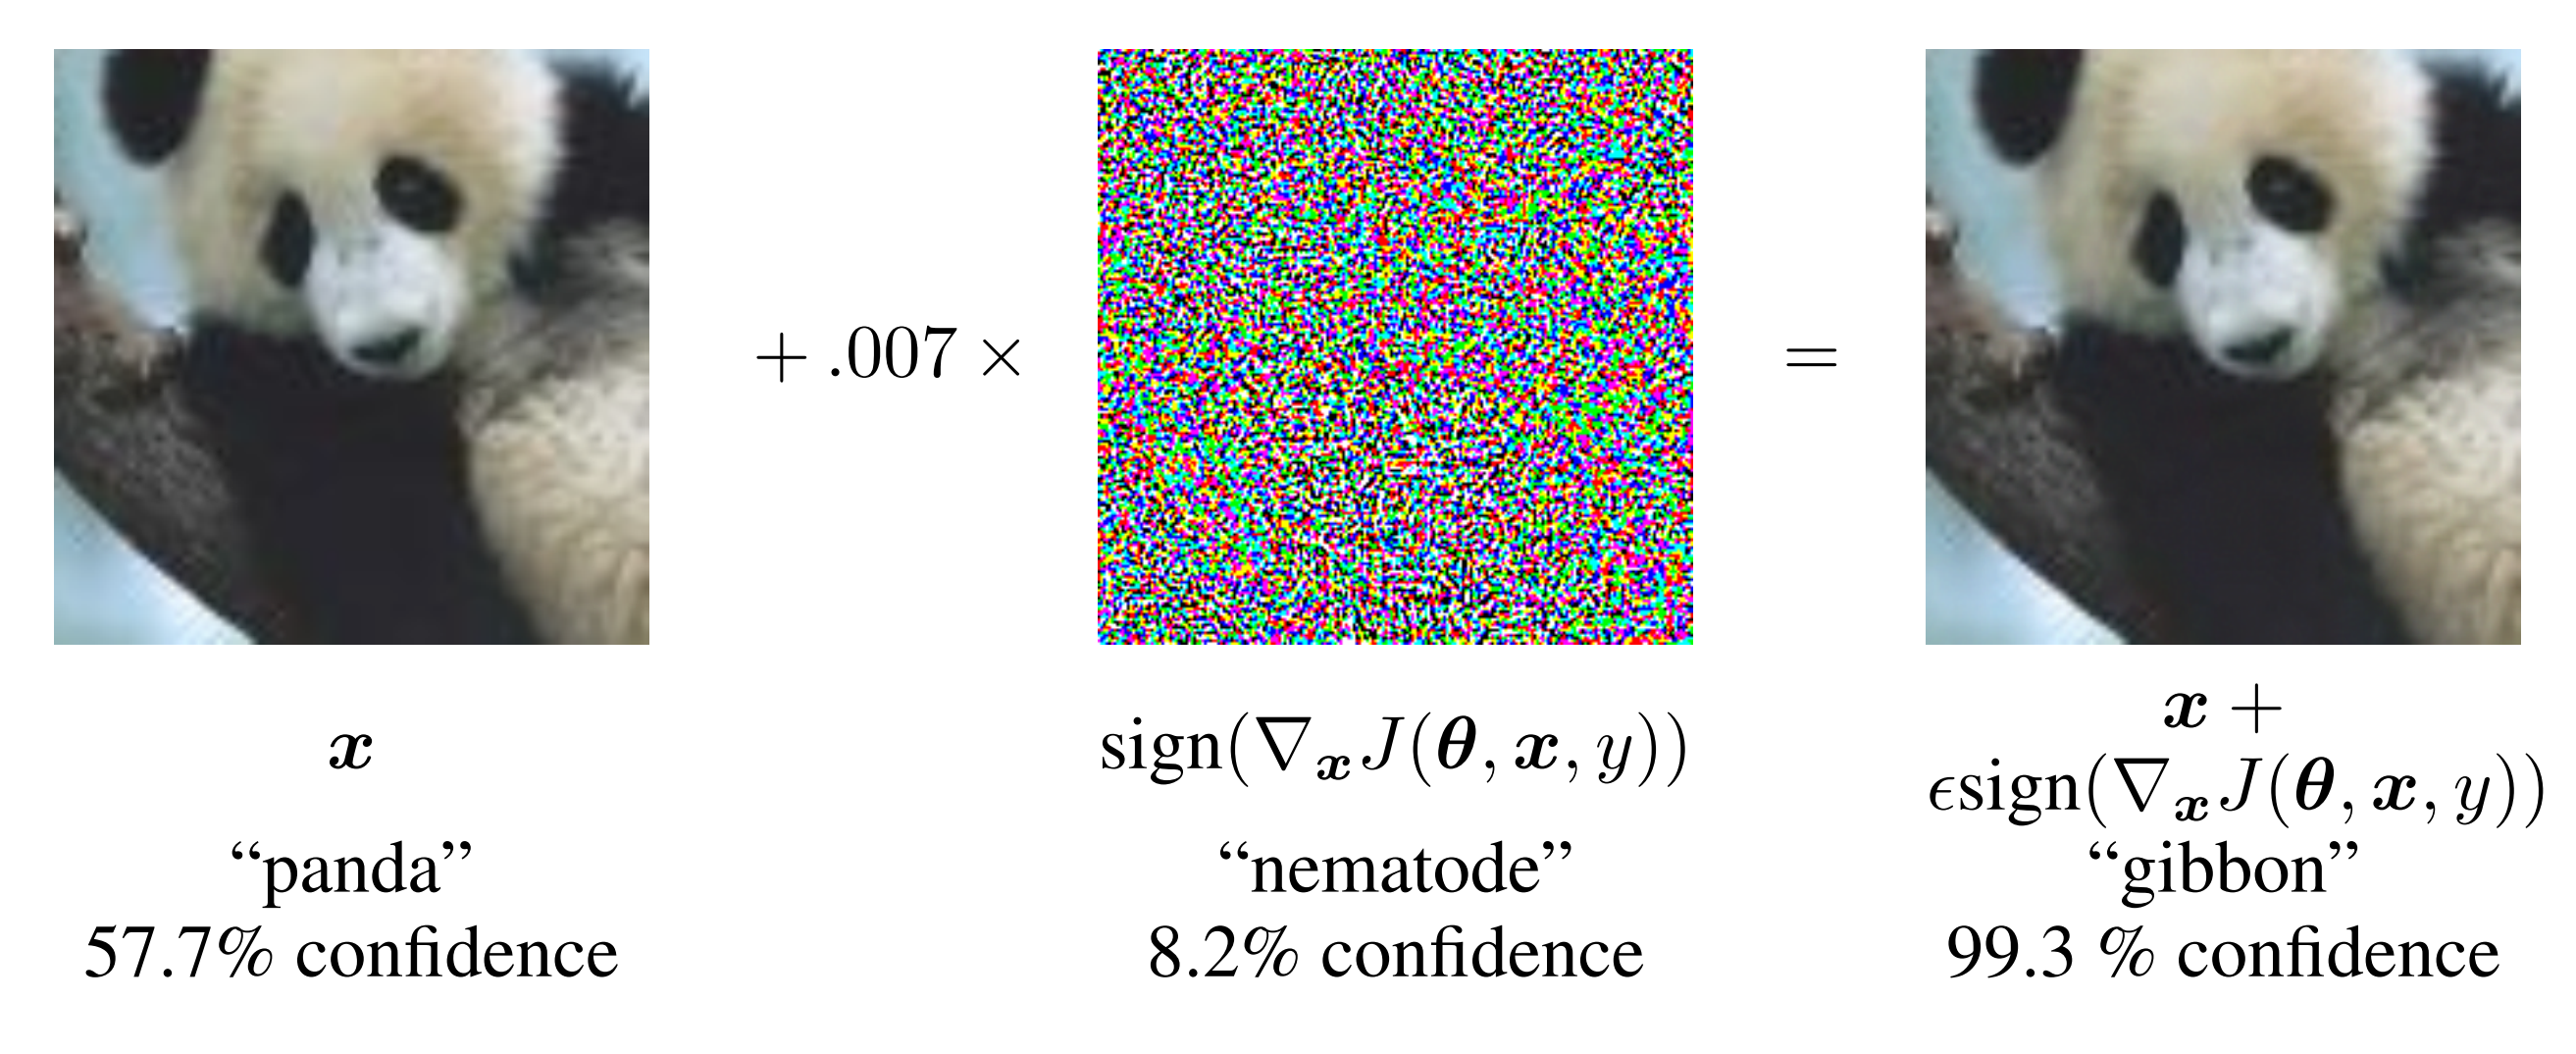
\includegraphics[width=0.7\linewidth]{panda_gibbon.png}
    \caption{Classic illustration of an adversarial example. A small perturbation that is nearly imperceptible to humans is added to an image of a panda. While the original image is correctly and confidently classified as a panda, the perturbed image is misclassified as a gibbon; also with high confidence. Adapted from \cite{goodfellow2014explaining}.}
    \label{fig:panda_gibbon}
\end{figure}

\begin{definition}[Adversarial Example]
An \textit{adversarial example} is an \textbf{input to a machine learning model} that has been \textbf{intentionally perturbed}, typically \textbf{in a subtle and often imperceptible manner}, such that the model produces an incorrect prediction while the semantic content of the input remains unchanged.
\end{definition}

\paragraph{Machine Learning Models.}
While adversarial examples are most commonly studied in the context of deep neural network classifiers~\cite{szegedy2013intriguing,madry2017towards,pitropakis2019taxonomy}, the phenomenon is not limited to neural networks. Adversarial vulnerabilities have been demonstrated across a wide range of machine learning architectures, including decision trees, support vector machines, $k$-nearest neighbour classifiers, logistic regression models, ensemble methods and more. This suggests that susceptibility to adversarial manipulation is a property of machine learners in general rather than a characteristic of a specific machine learning method~\cite{papernot2016distillation, szegedy2013intriguing, goodfellow2014explaining}.

\paragraph{Intentional Perturbations.}
The requirement that perturbations are \textit{intentional} reflects the modern understanding of adversarial examples. The seminal work of Szegedy et al. \cite{szegedy2013intriguing} demonstrated the existence of inputs that caused misclassification despite appearing unchanged to humans, but did not initially frame these inputs primarily as the result of a deliberate attack. As the field evolved, researchers showed that such inputs can be generated systematically through optimisation procedures and exploited by an adversary~\cite{moosavi2016deepfool, madry2017towards}. Consequently, adversarial examples are now typically discussed in the context of \textit{adversarial attacks}, where perturbations are deliberately crafted to elicit faulty model behaviour~\cite{chakraborty2018adversarial, pitropakis2019taxonomy, costa2024deep}.

\paragraph{Subtle and Imperceptible Perturbations.}
The notion of \textit{subtlety} for such perturbations can be interpreted in two related but distinct ways. First, adversarial perturbations are commonly constrained to be mathematically small according to a chosen distance metric. These norms define the \textit{perturbation budget} available to an adversary and provide a mathematical notion of similarity between inputs. We will discuss these different norms in more detail in Section~\ref{sssec:norms}.

Second, adversarial examples are often understood to be imperceptible to humans. In the image domain, this means that the perturbed input should be visually indistinguishable or at least hardly distinguishable from the original image, preserving its semantic meaning~\cite{madry2017towards,moosavi2016deepfool}. Although we rarely see the perceptibility of the applied perturbations rigorously validated it is nevertheless very common for authors to state, based on a visual assessment, that the adversarial examples they have generated are indistinguishable from the original to humans~\cite{brendel2017decision, chakraborty2018adversarial, costa2024deep, liang2022adversarial, papernot2016distillation, papernot2016transferability}.

\subsection{Taxonomy}
\label{sec:taxonomy}

Adversarial attacks can be categorised according to several orthogonal dimensions which we are presenting in this section. These dimensions are widely used throughout the literature and provide a useful framework for comparing attack methodologies~\cite{pitropakis2019taxonomy,costa2024deep}. The attacks discussed in this survey are classified according to this taxonomy, with a complete overview provided in Table~\ref{table_with_all_attacks}.

\subsubsection{By Attacker Knowledge}

One of the most common distinctions is based on the amount of information available to the attacker about the target model~\cite{pitropakis2019taxonomy,costa2024deep}.

\paragraph{White-box Attacks.}
In a \textit{white-box} setting, the attacker has complete knowledge of the target model, including its architecture, parameters, training procedure, and gradients. This level of knowledge makes highly effective optimisation-based attacks possible that directly exploit gradient information to identify adversarial perturbations. Many influential attacks, including the Fast Gradient Sign Method (FGSM), Projected Gradient Descent (PGD), and the Carlini-Wagner attack, were originally proposed in this setting. White-box attacks are commonly used to evaluate the worst-case robustness of machine learning models.

\paragraph{Black-box Attacks.}
In a \textit{black-box} setting, the attacker has no knowledge about the internal structure of the model and can only observe its outputs in response to supplied inputs. Such attacks more closely resemble many real-world scenarios, where proprietary models are exposed only through prediction interfaces or APIs.

\subsubsection{By Attack Stage}

Attacks can further be classified according to the stage of the machine learning pipeline at which they are carried out~\cite{chakraborty2018adversarial,pitropakis2019taxonomy}.

\paragraph{Evasion Attacks.}
\textit{Evasion attacks} are performed during the inference phase after a model has been trained. The attacker modifies input samples in order to induce misclassification while avoiding detection. Since such attacks they require no influence over the training process, they are considered the most practical and widely studied form of adversarial attack.

\paragraph{Poisoning Attacks.}
\textit{Poisoning attacks} target the training phase by injecting maliciously crafted samples into the training dataset. The objective here can be degradeing the model's overall performance, manipulating its behaviour for specific inputs, or implant hidden backdoors that can later be triggered by an attacker. While poisoning attacks require some influence over the data collection or training pipeline, this assumption is realistic in settings that rely on crowdsourced, user-generated, or automatically collected data.

\subsubsection{By Attack Goal}

The third dimension considers the attacker's intended outcome~\cite{chakraborty2018adversarial,costa2024deep,brendel2017decision}.

\paragraph{Targeted Attacks.}
\textit{Targeted attacks} seek to persuade the model to produce a specific attacker-chosen output. Drawing on the example given in \ref{fig:panda_gibbon}, an attacker might attempt to modify an image of a panda such that it is classified as a gibbon. Because the attack must drive the prediction toward a particular target class, targeted attacks are generally more difficult to perform than untargeted attacks.

\paragraph{Untargeted Attacks.}
\textit{Untargeted attacks} aim only to cause a prediction error, but do not specify the resulting incorrect class. The attack is therefore successful as soon as the model's prediction differs from the correct label. Again using the example from \ref{fig:panda_gibbon}, the attacker might aim at having the classifier recognize the perturbed image as showing anything but a panda.

\subsubsection{By Perturbation Constraint}
\label{sssec:norms}
Adversarial attacks are commonly categorised according to the distance metric used to constrain the perturbation applied to the input~\cite{costa2024deep, liang2022adversarial}. These constraints define what constitutes a \textit{small} modification and therefore determine the attacker's search space~\cite{carlini2017towards}. The majority of attacks in the literature operate under one of three norm-based threat models. Figure~\ref{fig:norms} illustrates these three norms geometrically.

\begin{figure}
    \centering
    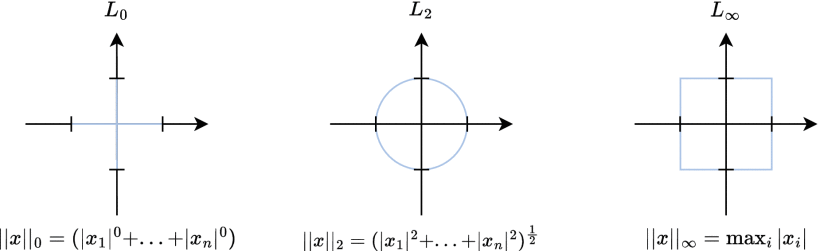
\includegraphics[width=0.7\linewidth]{norms.png}
    \caption{Geometric interpretation of the three norm constraints commonly used in adversarial machine learning. The unit balls of the $L_0$, $L_2$, and $L_\infty$ norms are shown in a two-dimensional feature space. The $L_0$ norm constrains the number of modified features, the $L_2$ norm constrains the Euclidean distance between the original and perturbed input, and the $L_\infty$ norm constrains the maximum change applied to any individual feature. Figure adapted from \cite{costa2024deep}.}
    \label{fig:norms}
\end{figure}

\paragraph{$L_0$-Constrained Attacks.}
The $L_0$ norm measures the number of features that have been modified. In the context of image classification, this corresponds to the number of altered pixels regardless of the magnitude of the changes. An example is the $L_0$ variant of the Carlini-Wagner attack~\cite{carlini2017towards}.

\paragraph{$L_2$-Constrained Attacks.}
The $L_2$ norm measures the Euclidean distance between the original and perturbed input vectors. Under this constraint, perturbations may be distributed across many features as long as the overall magnitude remains small~\cite{liang2022adversarial}. Due to its intuitive geometric interpretation, the $L_2$ norm is widely used when evaluating adversarial robustness~\cite{costa2024deep}.

\paragraph{$L_\infty$-Constrained Attacks.}
The $L_\infty$ norm limits the maximum change that can be applied to any individual feature~\cite{costa2024deep, liang2022adversarial}. Many influential attacks, including \textit{FGSM} and \textit{PGD}, operate under an $L_\infty$ constraint because it provides a straightforward approximation of perceptual similarity while enabling efficient optimisation~\cite{goodfellow2014explaining,madry2017towards}.

\subsection{Notable Evasion Attacks}
This section presents several notable adversarial attacks that have significantly influenced the development of the research area. An overview of these attacks, together with their classification according to the taxonomy introduced in Section~\ref{sec:taxonomy}, is provided in Table~\ref{table_with_all_attacks}. %Throughout the following sections we follow the notation of the respective original papers; the same symbols (e.g.\ $\delta$, $\epsilon$, $\eta$, $f$) may therefore denote different quantities in different subsections.

\begin{table}[t]
\centering
\caption{Overview of the attacks discussed in this survey, classified along the four dimensions of the taxonomy in Section~\ref{sec:taxonomy}. ``Both'' marks attacks with widely used targeted and untargeted variants; ``-'' marks poisoning attacks for which an input-space norm budget does not directly apply.}
\label{table_with_all_attacks}
\small
\begin{tabular}{@{}lcccc@{}}
\toprule
Attack & Knowledge & Stage & Goal & Constraint \\
\midrule
L-BFGS~\cite{szegedy2013intriguing}                     & White-box & Evasion   & Targeted   & $L_2$ \\
FGSM~\cite{goodfellow2014explaining}                    & White-box & Evasion   & Untargeted & $L_\infty$ \\
BIM / iterative~\cite{kurakin2017physical}              & White-box & Evasion   & Both       & $L_\infty$ \\
PGD~\cite{madry2017towards}                             & White-box & Evasion   & Untargeted & $L_\infty$ \\
DeepFool~\cite{moosavi2016deepfool}                     & White-box & Evasion   & Untargeted & $L_2$ \\
Carlini-Wagner~\cite{carlini2017towards}               & White-box & Evasion   & Targeted   & $L_0/L_2/L_\infty$ \\
ZOO~\cite{chen2017zoo}                                  & Black-box & Evasion   & Both       & $L_2$ \\
BadNets~\cite{gu2017badnets}                            & White-box & Poisoning & Targeted   & - \\
Targeted backdoor~\cite{chen2017targeted}               & Black-box & Poisoning & Targeted   & - \\
Poison Frogs~\cite{shafahi2018poison}                   & White-box & Poisoning & Targeted   & - \\
Clean-label backdoor~\cite{turner2019label,saha2020hidden} & White-box & Poisoning & Targeted & - \\
Narcissus~\cite{zeng2023narcissus}                      & Black-box & Poisoning & Targeted   & $L_\infty$ \\
\bottomrule
\end{tabular}
\end{table}

\subsubsection{L-BFGS}
The first widely recognised adversarial attack was introduced by Szegedy et al.~\cite{szegedy2013intriguing}. Their work did not only show that machine learning models are vulnerable to inputs that lead to incorrect predictions while appearing unchanged to human observers, first describing the phenomenon of an adversarial example. They furthermore introduced a first reliable method to find such examples.

To generate adversarial examples, the authors formulated the problem as a constrained optimisation task. Given an input $x$ and a target class $t$, the objective is to find the smallest perturbation $\delta$ such that the perturbed input $x+\delta$ is classified as the target class:

\begin{equation}
\min_\delta \|\delta\|_2
\quad \text{subject to} \quad
f(x+\delta)=t,
\end{equation}

where $f$ denotes the classifier and $\|\delta\|_2$ represents the Euclidean distance between the original and perturbed input. 
Directly solving this problem is difficult since the classification constraint $f(x+\delta)=t$ is highly non-linear and non-convex. To make the problem handleable, Szegedy et al. reformulated it as a continuous optimisation problem by replacing the hard classification constraint with a differentiable loss term that encourages the model to predict the target class. Specifically, they minimise

\begin{equation}
\min_\delta \; c\|\delta\|_2 + L_f(x+\delta,t),
\end{equation}

subject to the box constraint

\begin{equation}
x+\delta \in [0,1]^m,
\end{equation}

where $L_f(x+\delta,t)$ measures how strongly the network predicts class $t$. The parameter $c>0$ controls the trade-off between achieving the target misclassification and keeping the perturbation small, and the box constraint ensures that the perturbed input remains a valid image. This reformulation yields a differentiable objective whose gradients can be computed via backpropagation, allowing the perturbation to be found efficiently using the box-constrained Limited-memory Broyden-Fletcher-Goldfarb-Shanno (L-BFGS) optimisation algorithm. A line search over $c$ is then performed to identify the smallest successful perturbation that causes the classifier to output the target class.

Although the L-BFGS attack is still computationally expensive compared to later methods, its significance lies in motivating the extensive research that followed. For this reason, it is widely regarded as the starting point of adversarial machine learning research~\cite{goodfellow2014explaining, costa2024deep, liang2022adversarial}.

\subsubsection{Fast Gradient Sign Method (FGSM)}\label{sssec:fgsm}
Goodfellow et al.\ hypothesized that the reason adversarial examples exist is that commonly, models are designed to behave mostly linear \cite{goodfellow2014explaining}. Previously, it was suspected that models were too non-linear \cite{szegedy2013intriguing}.

Based on this hypothesis, they came up with the fast gradient sign method to find $L_\infty$-constrained adversarial examples. $L_\infty$ is chosen because it models sensor inaccuracies: a small perturbation in a sensor value would still be encoded to the same digital value.%Under their reasoning that models are mostly linear, the functions they represent are mostly linear as well. That means that we can approximate them around a point x in input space using the gradient. Goodfellow et al %hypothesize that the cost function around this point also can be approximated this way since it (why??? How does this follow from before??)(This assumes that the cost function [...?] is mostly smooth? WARNING: MIGHT NOT BE 100% REASONABLE! ->PGD / is debateable). (when? go into detail!)
Unlike L-BFGS, they did not choose a specific target class they want the adversarial example to be mistaken for. Instead, they aim to maximise the loss value of the adversarial example. That means that we want to solve 

\[\arg\max_{x' s.t. \lvert \lvert x'-x \rvert \rvert_\infty \leq \epsilon} L_f(x', y) = x + \arg\max_{\lvert\lvert\delta\rvert\rvert_\infty\leq\epsilon}L_f(x+\delta, y)\]

given a data point \(x\), a limit \(\epsilon\), and a loss function \(L_f(x, y)\) for the classifier \(f\), to find the 'worst' adversarial example (maximises loss) in the $L_\infty$-ball around $x$
%\todo{cost vs loss function?? Rewrite without x', but with epsilon?}

To do that, Goodfellow et al. linearise the loss function around $x$, giving us 

\[
\arg\max_{\lvert\lvert\delta\rvert\rvert_\infty\leq\epsilon}L_f(x+\delta, y) = 
\arg\max_{\lvert\lvert\delta\rvert\rvert_\infty\leq\epsilon}L_f(x, y) + \nabla_x L_f(x, y)^T \delta =
\arg\max_{\lvert\lvert\delta\rvert\rvert_\infty\leq\epsilon}\nabla_x L_f(x, y)^T \delta
\]
%\[\max_{x' s.t. \lvert \lvert x'-x \rvert \rvert_\infty \leq \delta} L(\theta, x', y) = \max_{x' s.t. \lvert \lvert x'-x \rvert \rvert_\infty \leq \delta} L(\theta, x, y) + \nabla_x L(\theta, x, y)^T (x'-x) =L(\theta, x, y)\max_{\lvert\lvert\eta\rvert\rvert_\infty\leq\delta}\]%\[= \arg\max_{x' s.t. \lvert \lvert x'-x \rvert \rvert_\infty \leq \delta} \nabla_x L(\theta, x, y)^T x'\]
%Choosing $\eta = \delta \cdot sign(\nabla_x L(\theta, x, y))$ is a valid maximiser, corresponding to a step in the direction of the sign of the gradient. \todo{reword this} This is why ... is known as the gradient sign method... results...
We can easily see that $\delta = \epsilon \cdot sign(\nabla_x L_f(x, y))$ is a valid maximiser of the scalar product  $\nabla_x L_f(x, y)^T \delta$. This corresponds to a single, as large as possible step in the direction of the gradient.

%It revolves around linearising the cost function $L(\theta, x, y)$ around a point $x$ in input space to maximise it.

%extend this to approximating the cost function using a gradient in the same manner. 

%Maximising ||x-x'||... gives us x_adv = ...

%This yielded good experimental results [cite], though later literature [cite PGD] improved results by not linearising the cost function as strictly.
%The method also yielded good results... \todo{"good"??} but worse than L-BFGS (cite DVERSARIAL MACHINE LEARNING AT SCALE)

Since this approach only needs one backpropagation step instead of iterations like an L-BFGS algorithm run, this was called the Fast Gradient Sign Method. It made adversarial training feasible, which aims to improve a model's robustness by inserting adversarial examples into the training set.

\subsubsection{Variants of FGSM}
%\todo{One-step target class meths, cf DVERSARIAL MACHINE LEARNING AT SCALE}

Different variants of FGSM were proposed by Kurakin et al.~\cite{kurakin2016adversarial, kurakin2017physical}.

The so-called \textbf{basic iterative method} applies FGSM multiple times with a small step size \cite{kurakin2017physical}. The adversarial example is given by
\[
x_{0}^{adv} = x, \quad x_{N+1}^{adv} = Clip_{x,\epsilon}
(
x_{N}^{adv} + \alpha \cdot sign(\nabla_x L_f(x_{N}^{adv} , y))
)
\]
where \(Clip_{x,\epsilon}\) implements pixel-wise constriction to the \(\epsilon\)-neighborhood of \(x\) \cite{kurakin2017physical}.

To find adversarial examples of a specific class \(t\) instead of maximising the loss function, FGSM can be modified to maximise that classes probability \(p(t | x)\). This can be achieved with a single step in direction of \(sign(\nabla_x \log(p(t | x)))\) \cite{kurakin2017physical}
%loss function formulation for Crossentropy
, analogous to basic FGSM, or using multiple, like in the aforementioned basic iterative method \cite{kurakin2016adversarial}. As target class, the one originally deemed least likely by the target model can be used. 




\subsubsection{PGD} \label{PGD}
%Like FGSM, adversarial attacks using projected gradient descent (PGD) as proposed by Madry et al. \cite{madry2017towards} use first-order information, i.e. the gradient of the loss function, but extend it to ... 
Searching adversarial examples by using projected gradient descent (PGD) as proposed by Madry et al. \cite{madry2017towards} is similar to the basic iterative method. Both use first-order information, i.e. the gradient of the loss function, to iteratively maximise the loss on an input in the neighborhood of the real image.
Instead of using multiple FGSM steps, though, Madry et al. use projected gradient descent directly. 

They formulate the adversary's goal as
\[
\max_{\delta\in S}L_f(x+\delta, y)
\]
%\todo{include the dual formulation? Not that important for adv. attacks?} 
Note the similarities to FGSM, by using \(S=\{\delta \mid \lVert \delta \rVert_\infty \leq \epsilon\}\), we obtain its maximization problem. FGSM is therefore a specific method to tackle this general formulation.

As a generalised, stronger attack, they propose using PGD. They support their argument with an experiment, starting PGD from random points in the vicinity of \(x\). While many different local maxima are found, they have roughly the same loss value. If an even better maximum existed, they argue, it would be hard to find with any first-order method. Therefore, no other first-order method could find it in reasonable time either, making PGD a useful "universal" first-order adversary.

However, this strength has a caveat. As we will see with momentum-based attacks later in this section ~\ref{sssec:momentum}, not every adversarial example corresponding to a local minimum is equally transferable to other models.

%This also ties into adversarial training [dual formula]..?
%-saddle point formulation (into theory part??) -> adversary goal, L norm flexibility, FGSM as special case

%others 
%ADVERSARIAL MACHINE LEARNING AT SCALE, e.g. basic iterative meth, One-step target class methods!!


%\begin{comment}
\subsubsection{DeepFool}
 DeepFool was introduced by Moosavi-Dezfooli et al.~\cite{moosavi2016deepfool} in 2016. The central idea of this iterative method is to characterise adversarial vulnerability geometrically: rather than loosely optimising an attack loss, DeepFool estimates the distance of an input to the closest decision boundary. For affine classifiers, this distance could be calculated in a closed form by projecting the input point onto the decision hyperplane. Moosavi-Dezfooli et al. suspect that deep neural networks have highly nonlinear decision boundaries, contrary to Goodfellow et al.'s argumentation. These boundaries are addressed by DeepFool by exploiting the observation that although the true boundary of a neural network may be highly curved, sufficiently small neighborhoods can often be approximated accurately by a hyperplane. The shortest path to this approximate boundary is assumed to provide a good estimate of the minimal adversarial perturbation. This auxiliary hyperplane is recomputed at each iteration through a first-order Taylor expansion of the classifier around the current point; as the point is repeatedly projected onto the latest hyperplane, it moves closer and closer to the true, nonlinear decision boundary until it eventually crosses it. In mathematical terms, at an intermediate point $x_i$, the classifier is iteratively displaced by its local linear approximation,                                   

\begin{equation}
    f(x) \approx f(x_i) + \nabla f(x_i)^T(x-x_i),
\end{equation}

which defines a locally linear decision boundary. The perturbation is obtained by projecting the current point onto this locally estimated boundary, yielding an update

\begin{equation}
    x_{i+1}=x_i+\delta_i,
\end{equation}

where $\delta_i$ is the smallest perturbation that crosses the linearised boundary. The procedure is repeated until the classifier changes its prediction.

For multiclass classifiers, DeepFool extends this idea by considering the set of pairwise decision boundaries between the current class and competing classes. At each iteration, the method computes the locally closest boundary under the linear approximation and updates the input toward that boundary. Figure~\ref{fig:deepfoolmulticlasslinearapproximation} visualises the iteration step.

\begin{figure}
	\centering
	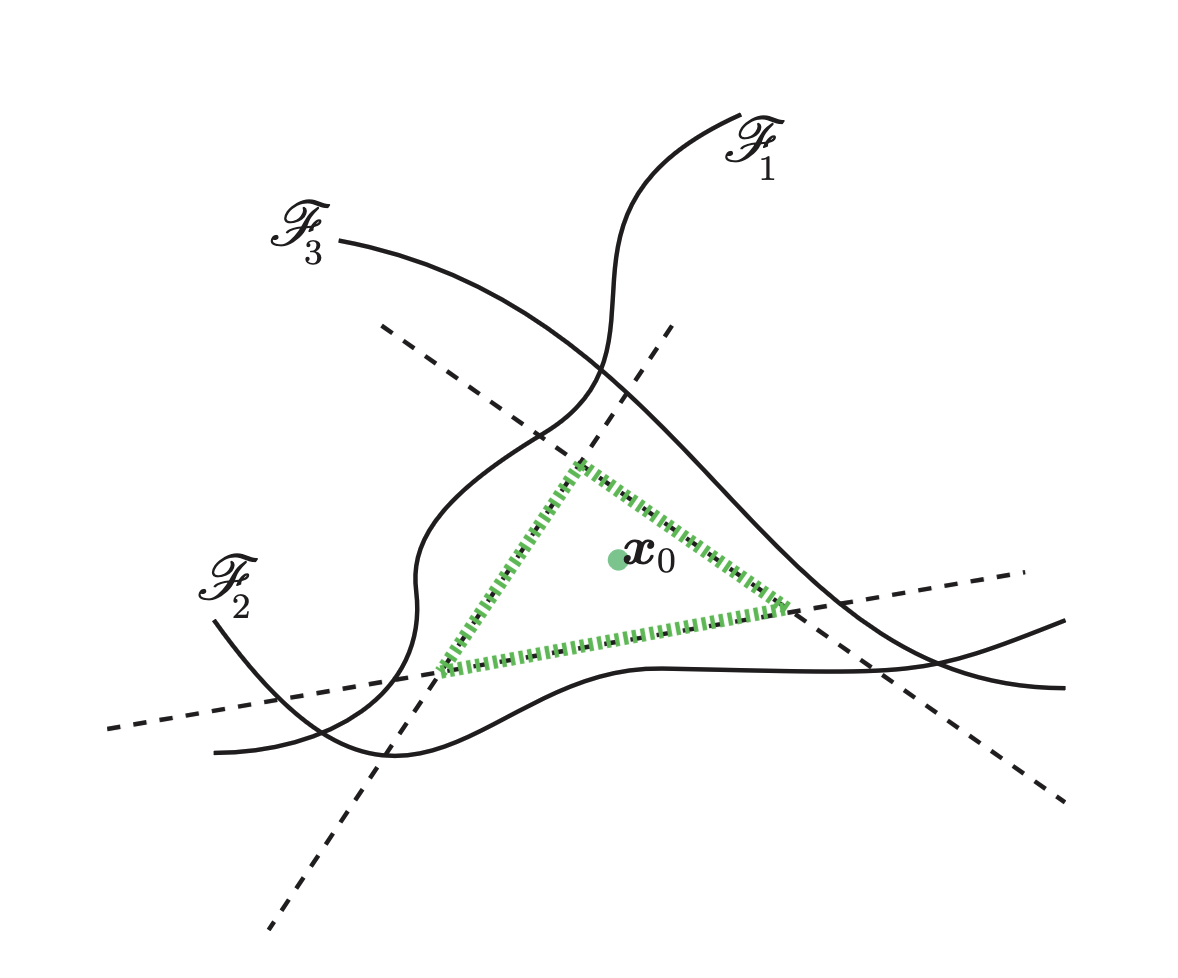
\includegraphics[width=0.4\linewidth]{deepfool_multiclass_linear_approximation}
	\caption{The approach of DeepFool estimates the position of the decision boundaries with the other classes with a linear representation using first-order Taylor expansion. By iteratively projecting the input point onto this auxiliary hyperplane, the perturbed point moves closer and closer to the actual decision boundary of the model until eventually crossing it.}
	\label{fig:deepfoolmulticlasslinearapproximation}
\end{figure}

Maybe the most important contribution of DeepFool to the  field of adversarial attacks is the geometrical perspective that it shed on the problem: instead of treating adversarial generation as a generic constrained optimisation problem, it directly exploits the local structure of the classifier and latches onto a geometrical image of the decision boundary that needs to be crossed. Furthermore, it gave the L-BFGS attack of Szegedy et al.~\cite{szegedy2013intriguing} a new, which had required solving a computationally expensive optimisation problem for each input. By using gradient information to directly estimate the boundary geometry, DeepFool achieved smaller perturbations than earlier methods while requiring considerably less computation than general-purpose optimisation approaches.

\subsubsection{Carlini-Wagner}
The Carlini-Wagner (C\&W) attack is an influential attack presented by Carlini and Wagner~\cite{carlini2017towards}. The method builds directly upon the original L-BFGS method by Szegedy et al.~\cite{szegedy2013intriguing} by substantially improving the objective function of the optimisation problem. They further introduced a trick to formulate the problem as an unconstrained optimisation task, instead of a constrained one.

Just like L-BFGS, given an input example $x$ and a target class $t$, the attack seeks an adversarial example $x'=x+\delta$ by solving:

\begin{equation}
\min_{\delta} \|\delta\|_p + c \cdot l(x+\delta),
\end{equation}

where $\|\delta\|_p$ measures the size of the perturbation and $l$ is a logit-based loss function that operates on the network's raw logits rather than the softmax output probabilities. The loss is defined as:

\begin{equation}
l(x') =
\max \left(
\max_{i \neq t} z_i(x') - z_t(x'),
-k
\right),
\end{equation}

where $z_i(x')$ denotes the logit corresponding to class $i$, and $k$ is a confidence parameter controlling the margin by which the target class must exceed competing classes. This formulation directly optimises against the decision boundary of the classifier and thus efficiently calculates adversarial examples.

To address the pixel-range constraint of image inputs, the C\&W attack introduces a clever variable transformation:

\begin{equation}
x'=\frac{1}{2}(\tanh(w)+1),
\end{equation}

where $w$ is an unconstrained latent space optimisation variable. This transformation converts the original constrained optimisation problem into an unconstrained one while guaranteeing that the generated adversarial example remains within the valid input range. The attack then optimises $w$ using gradient-based optimisation methods, typically the Adam optimiser~\cite{kingma2014adam}.

The original work introduced variants based on different distance metrics, including $L_0$, $L_2$, and $L_\infty$ norms, allowing the attack to evaluate robustness under different threat models.

The effectiveness of the C\&W attack also demonstrated weaknesses in several proposed defenses. In particular, it was shown to successfully bypass defensive distillation \cite{papernot2016distillation}, a technique proposed to improve adversarial robustness by training a model using softened output probabilities from a teacher network. Although defensive distillation appeared to increase resistance against earlier attacks, Carlini and Wagner demonstrated that the method did in fact only obscure the model's gradient albeit not truly hiding it. By directly targeting the logits with their loss function, Carlini and Wagner were able to efficiently generate adversarial examples in spite of defensive distillation by directly approximating the obscured decision boundary.
%\end{comment}

%\subsubsection{Transfer Attacks}


\subsubsection{Jacobian-Based Dataset Augmentation}
In a transfer attack, an adversary first creates and trains a substitute model as a stand-in for a target black-box model that he has full access to. On this substitute, white-box attacks like the ones described above can be performed to find adversarial examples. Since they generally transfer from one model to another, these can then be used to attack the actual target model.
Papernot et al. \cite{papernot2017practical} introduced black-box attacks via transfer attacks where neither target model parameters nor a suitable data set is accessible to the attacker. Prior work by Biggio et al.\ \cite{biggio2013evasion} had introduced transfer attacks already, but granted access to such a dataset.

Papernot et al. address the dataset restriction by querying the target on artificial data points to create a substitute dataset. Here, the selection of good data points to learn similar decision boundaries is crucial: a bad crafting strategy would require infeasible and highly suspicious amounts of queries to the target model. In particular, generation based on random noise does not work.
Instead, they rely on a heuristic to find out in which input direction the (substitute!) model's output changes and adding new samples focused on these directions. For that, they rely on the substitute model's Jacobian matrix (multidimensional derivative, each entry is one output coordinate partially derived by an input coordinate) at input points.

The first step is collecting a set of samples somewhat representative of the target's input domain, such as different natural images. After, the substitute architecture is defined based on input and output of the target, e.g. one adapted to images. The architecture is overall not a deciding factor in the success of this approach.
The following steps are then performed repeatedly: The adversary makes the target model label his current selection of samples, and then trains his substitute with the new examples. Next, he augments his dataset with additional input points:

Let \(J_f(x)\) be the Jacobian of the substitute at a point x. Then, \(J_f(x)[o(x)]\) is the column corresponding to partial derivatives of the correct label (i.e. the one assigned by the target model). Papernot et al. now add the sign of this column scaled by a factor \(\alpha\) to point x: \(x = x + \alpha \cdot sign(J_f(x)[o(x)])\), and add it to their dataset. The idea is to move the example along directions in which model output changes strongly, with the intuition that these directions need more samples to accurately model the target's decision boundaries.

By doing this to all current points, they obtain a larger sample set, so the model trained in the next iteration is closer to the target. Note that every epoch, the model is trained from scratch. With enough iterations, the substitute can then be used to generate the adversarial examples.
% !!! check Jacobian definition

\subsubsection{Ensemble Attacks}
For transferability attacks to work, it is crucial that adversarial examples constructed on the substitute model translate well to the target model. To improve this transferability, Liu et al. \cite{liu2016delving} argue that an adversarial example that works well for multiple models at the same time is bound to transfer better than one that only works on a single one.

They therefore propose that an adversary in the transfer attack setting crafts adversarial examples against an ensemble of models. For a targeted attack, they suggest the negative-log-likelihood-objective:

\[
x^{*} = \arg\min_{x'}{-\log((\sum_{i=1}^k \beta_i f_i(x')) \cdot \mathbb{1}_{t}) + \lambda \frac{\lVert x - x'\rVert_2}{\sqrt{N}}}
\]
where \(N\) is the number of dimensions, \(t\) is the target class, \(f_i(\cdot)\) is each models output, \(\beta_i\) scaling factors for each such that \(\sum_i\beta_i=1\), for example simply \(1/k\). As a whole, this formula balances maximizing the probability assigned to the target class (first part) and keeping the perturbation small (second part). The \(\sqrt{N}\) serves as a normalisation factor for different input dimensions.

\subsubsection{MI-FGSM and Momentum}
\label{sssec:momentum}
Kurakin et al. \cite{kurakin2016adversarial} remarked that, while iterative methods yield better results on a single attacked white-box model, single-step methods exhibit better transferability. They suspected that iterative methods overfit to parameters of the model.

To tackle this issue, Dong et al. \cite{dong2018boosting} proposed adding momentum to iterative methods such as iterative FGSM, leading to momentum iterative FGSM. This way, both the underfitting of basic FGSM as well as the overfitting of iterative FGSM is eased.

The gradient is updated as
\[
g_{N+1} = \mu \cdot g_N + \frac{\nabla_x L_f(x_N^{*}, y)}{\lVert \nabla_x L_f(x_N^{*}, y) \rVert_1}
\]
with \(\mu\) being the decay factor and the gradient being normalised to handle gradient magnitudes varying over iterations.

Accordingly, the sample is updated as
\[
x_{N+1}^{*} = x_N^{*} + \alpha \cdot sign(g_{N+1})
\]
\(\alpha\) being the step size.
For \(\mu=0\), this goes back to being normal FGSM. Note that this change is not restricted to FGSM, but can be applied to any iterative gradient-based method including targeted ones.


\subsubsection{ZOO}
In 2017, Chen et al. \cite{chen2017zoo} proposed Zeroth-Order Black Box Attacks (ZOO), a black-box attack without the use of a substitute model. This way, they avoided losses in transferability to the target and achieved comparable %\todo{elaborate} 
results to then-state of the art white box attacks.

This attack is possible if the adversary is allowed to query the target model, i.e. obtaining the confidence scores, $f(x)$ for an arbitrary $x$. This might be the case for a classification-as-a-service tool. Gradients and model configuration, however, are not available (black box).

To circumvent this restriction, Chen et al. estimate a pseudo-gradient using two queries per coordinate:
\[
\hat{g_i}
:= \frac{\partial l(x)}{\partial x_i}
\approx \frac{l(x + he_i) - l(x - he_i)}{2h}
\]
where \(l\) is a loss function based on the model's output and \(h\) is set to a small constant instead of approaching 0 like in the derivation formula.
Naively, this would suffice to estimate full gradients and perform gradient descent. However, this formula requires two evaluations per coordinate, $l(x + he_i)$ and $l(x - he_i)$, each incorporating  a query to the model. Since each pixel translates to three coordinates of input data, this is not a feasible approach.

Instead, Chen et al. perform stochastic coordinate descent, improving just a batch of coordinates at each step. This way, they do not need to estimate the full gradient each time, similar to how stochastic gradient descent only uses a batch of samples at each step. For the optimisation itself, they use ADAM or Newton's method.

Still, we need to find a suitable loss function \(l\). In fact, we can use different loss functions to adapt different white-box attacks. In their work, Chen et al. adapted the Carlini-Wagner attack. C-W's loss function performs on the raw logits of a model, an information inaccessible in the black-box case.

Instead, Chen et al. use the logarithm of the confidence scores as a proxy of sorts for the logits %\todo{argue} 
and obtain
\[
%f(x,t) = \max\left\{ \max_{i\neq t} \log[F(x)]_i - \log[F(x)]_t,-\kappa \right\}
l(x,t) = \max\{ \max_{i\neq t} \{\log[f(x)]_i\} - \log[f(x)]_t,-\kappa \}
\]
for targeted attacks and
\[
%f(x,t) = \max\left\{ \max_{i\neq t} \log[F(x)]_i - \log[F(x)]_t,-\kappa \right\}
l(x) = \max\{ \log[f(x)]_{y} - \max_{i\neq y} \{\log[f(x)]_i\} ,-\kappa \}
\]
for untargeted ones.
%\todo{mutually improve this with Carlini-Wagner}

%Additionally, they propose different measures to speed up optimisation even more \todo{...}

%In fact, ZOO is more of a technique to adapt white-box attacks, such as Carlini-Wagner, to black-box targets. The downside is longer processing times.% as this adaptation is done using pseudo-gradients estimated from function values.

%\todo{Newton method using Hessian, and other tricks}






%-NO substitute model! (Include substitute model approach!!)
%-input-output only!
%-'translates' white-box Carlini-Wagner
%-extendable to other white-box approaches (pseudo gradient)
%-coordinate descent for feasibility
\subsection{Notable Poisoning Attacks}

Poisoning attacks were already included in the early taxonomy of Barreno et al.~\cite{barreno2010security}, which clustered attacks on machine learning into exploratory and causative, analogous to our evasion and poisoning taxonomy.

The first poisoning attack that got greater attention was Biggio et al.'s gradient-based attack on Support Vector Machines~\cite{biggio2012poisoning}. Subsequently, more research was contributed, especially on attacks on neural networks.

%\subsubsection{Back-gradient optimisation}
%Muñoz-González et al. \cite{munoz2017towards} introduced poisoning 

\subsubsection{Backdoor Poisoning Attacks}
% !!! In an authentication system, a backdoor ...
With backdoor attacks on machine learning as proposed by Chen et al. \cite{chen2017targeted} % in the context of authentication systems, the adversary's goal is to introduce a backdoor for himself into the model, meaning a way to bypass the mechanism. More specifically, the adversary seeks to create backdoor instances, inputs that model will assign the wrong label (chosen by the adversary) to and thereby grant the adversary access.
and Gu et al. \cite{gu2017badnets}, the adversary's goal is to introduce a backdoor for himself into the model. While the performance on normal inputs is to be kept up, the model should react to specific inputs by misclassifying them, either generally, or targeted. These specific inputs carry a special pattern, the "key" or "trigger".

Gu et al. consider an adversary that has full access to the model or a base version of it. Namely, an ML-as-a-service provider (full access) and a provider of pretrained models (base version access). In both cases, the architecture is specified already, as well as a training set. A backdoor key pattern is chosen by the attacker. The adversary has to find model weights performing well on general samples from the set yet vulnerable to the backdoor.

For that, Gu et al. use training set poisoning, adding a fraction of training images to the dataset again, only with the trigger pattern included and the labels changed according to varying strategies. They did not yet derive a way to optimise poison samples, instead, pattern, label change formula and infected fraction need to be selected by the adversary. In general, their focus was on the feasibility rather than the exact attack procedure.

Chen et al. instead use a black-box threat model where the adversary does not have access to model architecture or training data and can only inject a small number of adversary samples including arbitrary labels, in contrast with the powerful adversary assumed by Gu et al. 

Backdoor keys may either be a single instance or a pattern added to instances. The former ("input-instance-key" strategy) allows injecting just very few poisoned examples while the latter ("pattern-key") can be used to craft adversarial examples from a wide range of inputs, which is often more useful to a hypothetical attack and resembles Gu et al.'s poisoning. 

In input-instance-key strategies, Chen et al. propose adding different noised versions of the key-to-be to the training set, each with the chosen label. The idea is to get the model to overfit to these.
In Pattern-key strategies, the adversary can blend a key pattern onto pictures, add an accessory, or blend in an accessory according to Chen et al.'s suggestions. The idea of the blending is to make the pattern harder to spot for humans. In any case, the perturbed sample is added to the dataset as poison. 
Like Gu et al.'s attack, theirs also depends on hyperparameter choices only, with the framework not optimising poisoning on its own. 

\subsubsection{Clean-Label Backdoor Attacks}
Notably, while the backdoor poisoning attack described by Chen et al. does not need access to the model, the adversary has to be able to assign arbitrary labels to samples, as does the one by Gu et al. However, this can be highly noticeable and alert human overseers to the attack or might just not be feasible in another way. Clean-label attacks  do not give such power to the adversary.

One such attack was proposed by Shafahi et al. \cite{shafahi2018poison}. In contrast to Chen et al.'s attack, the adversary does know the model parameters, which might happen if the target model is based on a pretrained, freely accessible one. His goal is to have a chosen target instance \(v\) misclassified without modifying it, e.g. getting a malware script to bypass a ML antivirus. 

First, he samples a base instance \(b\), such that its class, the "base class", is the one he wants the target instance to be classified as. With this, he crafts a poison instance $p$ by solving 
\[
p = \arg\min_x {\lvert \lvert g(x) - g(v) \rvert \rvert_{2}^2
+ \lambda \lvert \lvert x - b \rvert \rvert_{2}^2} 
\]
where \(g\) is the output of the networks second-to-last layer (i.e., the feature representation) and \(\lambda\) is a constant. The first term compares the target v and poison candidates x in feature space (the more similar, the better), and the second penalises difference from the base instance. The general idea is to find a poison instance close to b, therefore likely to be labeled the same, yet close to v in feature space (output of second-to-last layer), so v is treated the same as b by the model. %Shafahi et al. argue that a suitable x can be found due to f being supposedly highly nonlinear. 
For optimisation, two steps are iterated: First, a gradient step ("forward step"), then a step towards b ("backwards step").
%\todo{FAIL graphic - similar}

%\subsubsection{Clean-Label Backdoor Attacks}
Saha et al. \cite{saha2020hidden}
made an effort to combine the clean-label approach with backdoor poisoning attacks, albeit Turner et al. did the same a year earlier \cite{turner2019label}. Both also considered how to hide the trigger during poisoning to decrease the noticeability of the backdoor, though differently. Turner et al. manually select a "trigger amplitude", essentially an opaqueness. Saha et al., on the other hand, directly incorporate it into their optimisation and not even have the pattern itself in the poisoned instance. 
% !!! vielleicht doch nicht so ähnlich, die beiden? cf Narcissus

% !!! images here?
Saha et al. consider a threat model in which the adversary can add poison to a dataset the victim uses for fine-tuning a pretrained model, which the adversary has access to. The scenario is similar to the one described by Gu et al., with the difference that the adversary attacks the fine-tuning, not the pretraining.

The attack itself is similar to Shafahi et al.'s. The adversary samples a source \(s\) and a base image \(b\) from the data distribution. He then applies his trigger to the source, obtaining the patched source. Like before, the poison sample is optimised to be close to the base image in pixel space (so it probably receives the same label) while close to the patched source in feature space (so the model has difficulties distinguishing them). Note that the Saha et al. call the base image the "target" instead. Figure \ref{fig:HTBA} illustrates their approach.

Let \(\tilde{s}\) be the patched source, \(b\) the base, and \(\epsilon\) a small, chosen threshold. Saha et al. optimise
\[
\arg\min_x{\lvert \lvert g(x) - g(\tilde{s}) \rvert \rvert_{2}^2} \quad\quad \textbf{s.t.} \quad \lvert \lvert x - b \rvert \rvert_{\infty} < \epsilon
\]
to obtain the poisoned sample x. Again, \(g\) is the output of the second-to-last layer, the feature space representation.
% !!! go more in detail about this look on NNs: "only last layer decides"?
To optimise, they use projected gradient descent. However, in each optimisation step, a new randomly-patched source is selected so the backdoor generalises to arbitrary images and patch placements. %...% !!! ... multiple at once, 1:1 problem

\begin{figure}[t]
    \centering
    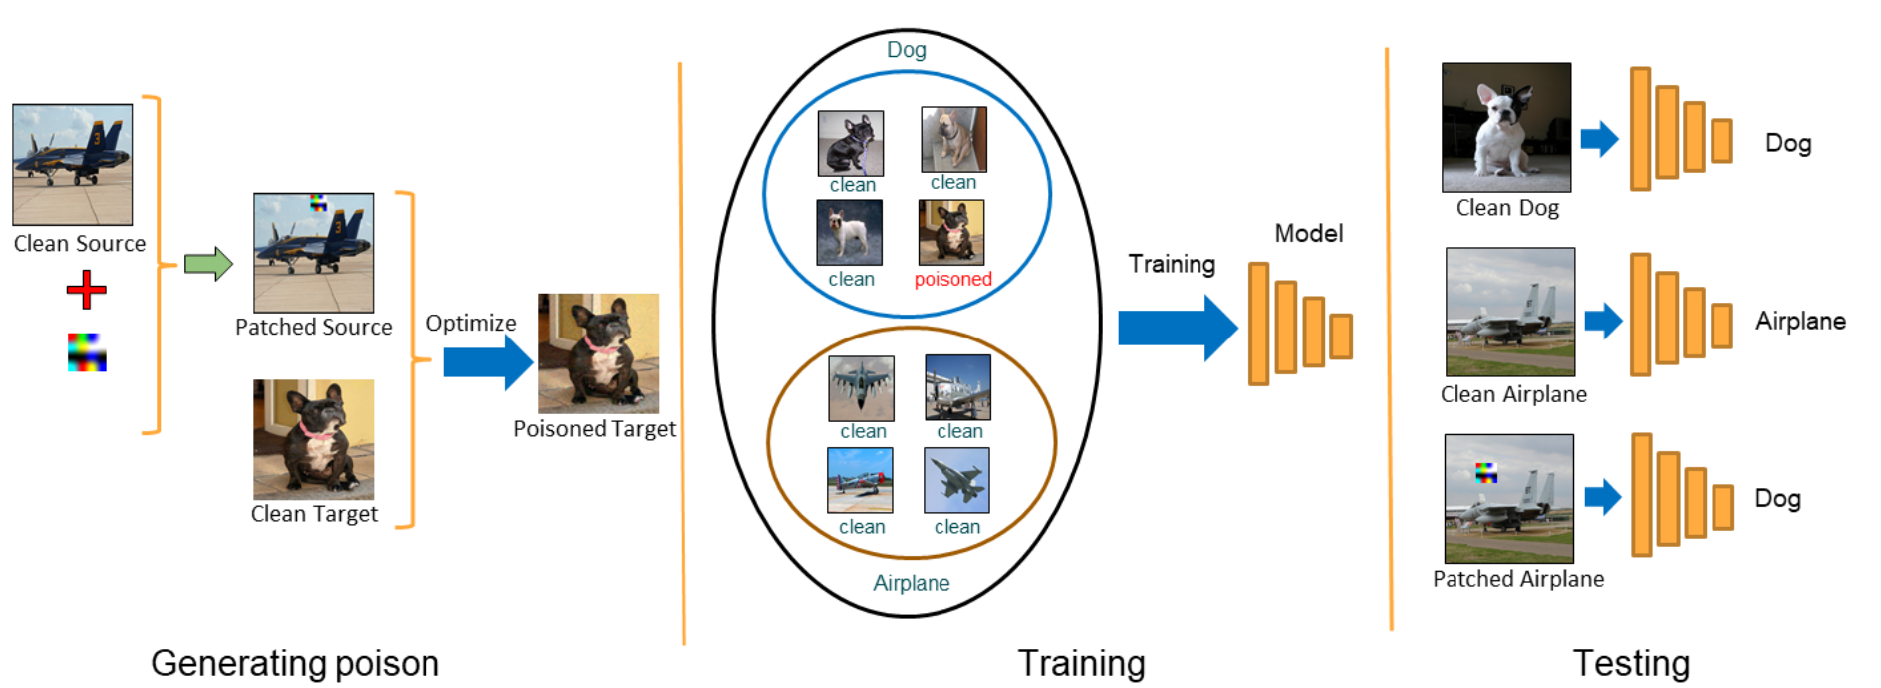
\includegraphics[width=1\textwidth]{HTBA_process.png}
    \caption{Saha et al.'s poisoning approach. \emph{Left:} A poisoned sample seeks to collide with the patched source in feature space while being close to the base (here: target) in pixel space. \emph{Middle:} The poison sample is added to the victim's dataset. \emph{Right:} In testing, the adversary can now apply the patch to images to have them misclassified.
    Taken from Saha et al. \cite{saha2020hidden}.}
    \label{fig:HTBA}
\end{figure}


%Narcissus, Label-consistent
A more recent work by Zeng et al. \cite{zeng2023narcissus} addresses the inefficiency of choosing arbitrary trigger patterns, while restricting the adversary further. 
They consider a black-box threat model where the adversary can only poison a small subset of the training data. The adversary chooses the target class \(t\) and knows some examples \(D_t\) in it. He also has general information on the task the victim model should perform, such as "face recognition", but not specifics like classes used. This enables the attacker to draw up more data instances related to the task, though they might not belong to the original data distribution and are therefore referred to as "public out of distribution (POOD) examples". This is especially easy in image or language tasks where lots of samples are available in the web.

Their approach revolves around optimising the trigger pattern used under a constraint so it is harder to notice for humans. Previous work had the adversary craft poisoning samples with an arbitrarily-choosen trigger (see above).
% !!! - Only some prior work was made on this, such as LIRA...
Suppose the attacker had access to the model the victim would obtain without poisoning. We call this model the oracle \(f_{orc}\). Recall that he also has access to a dataset of the target class \(D_t\). Zeng et al.'s approach is to choose a trigger \(\delta^{*}\) maximising the oracle's confidence on the target class, i.e. solving 
\[
\delta^{*} = \arg\min_{\delta\in S}{\sum_{(x,t)\in D_t}{L_{f_{orc}}(x+\delta, t)}}
\]
where \(S\) is the set of allowed perturbations, e.g. the \(L_\infty\)-ball. This way, \(\delta^{*}\) itself is related to the target class, and adding it to any input increases the likelihood of that input being classified as the target class. 
However, the adversary does not have access to \(f_{orc}\). Instead, Zeng et al. propose training a surrogate model \(f_{sur}\) on the POOD data \(D_{POOD}\). The above equation becomes
\[
\delta^{*} = \arg\min_{\delta\in S}{\sum_{(x,t)\in D_t}{L_{f_{sur}}(x+\delta, t)}}
\]

Now, the attack works as follows. First, \(f_{sur}\) is trained using \(D_{POOD}\) and \(D_t\).
While training the surrogate model on both \(D_{POOD}\) and \(D_t\) simultaneously would be possible, Zeng et al. suggest training on \(D_{POOD}\) first and fine-tune on \(D_t\) to make modification for a possible second attack on another class more efficient.
In the second step, they use (stochastic) projected gradient descent to find the trigger \(\delta^{*}\) and subsequently add it to a portion of the target class samples \(D_t\).
The victim is then given this poisoned target class data set.
In an eventual exploit, the adversary adds the trigger to the desired input. It is an option to amplify the trigger to increase attack success rates.
% !!! NArcissus - Zeng et al. \cite{zeng2023narcissus} 

% !!! all to one / one to one discussion??

%-Targeted Backdoor Attacks on Deep Learning
%Systems Using Data Poisoning
%->proposed Backdoor Attacks, Backdoor poisoning attacks (in blackbox?)

% !!! gradient / feature collision approach?? schon drin

% !!! important metrics for poisoning

\section{Discussion}
\label{sec:discussion}

As throughout this survey, the following discussion stays within the setting of image classification, which concentrates most of the research and, being inherently visual, affords readily interpretable illustrations of the phenomena at hand.

\subsection{Real-World and Physical Adversarial Attacks}

Somewhat surprisingly, in practice, confirmed \textit{malicious} adversarial-example attacks against real institutions or individuals remain strikingly rare~\cite{biggio2018wild, raff2023dont}. Two explanations seem possible. 

\begin{enumerate}
	\item Adversarial attacks slip through unnoticed: a successful adversarial input may be logged as an ordinary misclassification, be considered a generic model error, or filed under an unrelated incident category, so that successfully employed adversarial attacks fly under the radar.
	\item Adversarial attacks might in practice simply be of little use to actual attackers. Crafting them reliably demands specialised machine-learning and security expertise, whereas cruder techniques---distributed denial-of-service, character obfuscation to slip past spam filters, or merely packing a malware binary---remain cheap, fast, and effective~\cite{apruzzese2023real, raff2023dont}.
\end{enumerate}

 The second explanation is the one that we consider to be more plausible.  Building an adversarial example to defeat a system that a simpler attack would already defeat is like learning to pick a lock when the crowbar is cheaper, quicker, and works just as well. Interestingly, the few confirmed real-world cases, such as commercial CAPTCHA-solving services or the prompt injection of deployed chatbots, tend to be those where no such simpler alternative exists.

This does not render the phenomenon academic in the pejorative sense. As machine learning is embedded ever more deeply into the physical world---autonomous vehicles, automated border control, biometric surveillance---the question of whether an input that is semantically unchanged to a human can nonetheless fool a sensor pipeline becomes a central engineering concern. The body of work on \textit{physical} adversarial attacks shows that it can, as the examples in Figure~\ref{fig:physical} illustrate: inconspicuous stickers on a stop sign reliably cause targeted misclassification, both in the laboratory and from a moving vehicle~\cite{eykholt2018robust}; printable adversarial patches force a chosen label onto almost any scene they appear in~\cite{brown2017adversarial}; adversarial eyeglass frames defeat face recognition~\cite{sharif2016accessorize}; and spoofed sensor returns or crafted road-surface markings can mislead the perception stack of a production self-driving system~\cite{cao2019adversarial, tencent2019tesla}.

\begin{figure}[t]
	\centering
	\subcaptionbox{A 3D-printed turtle that is consistently misclassified as a rifle. Reproduced from \cite{athalye2018synthesizing}\label{fig:adversarialturtle}}{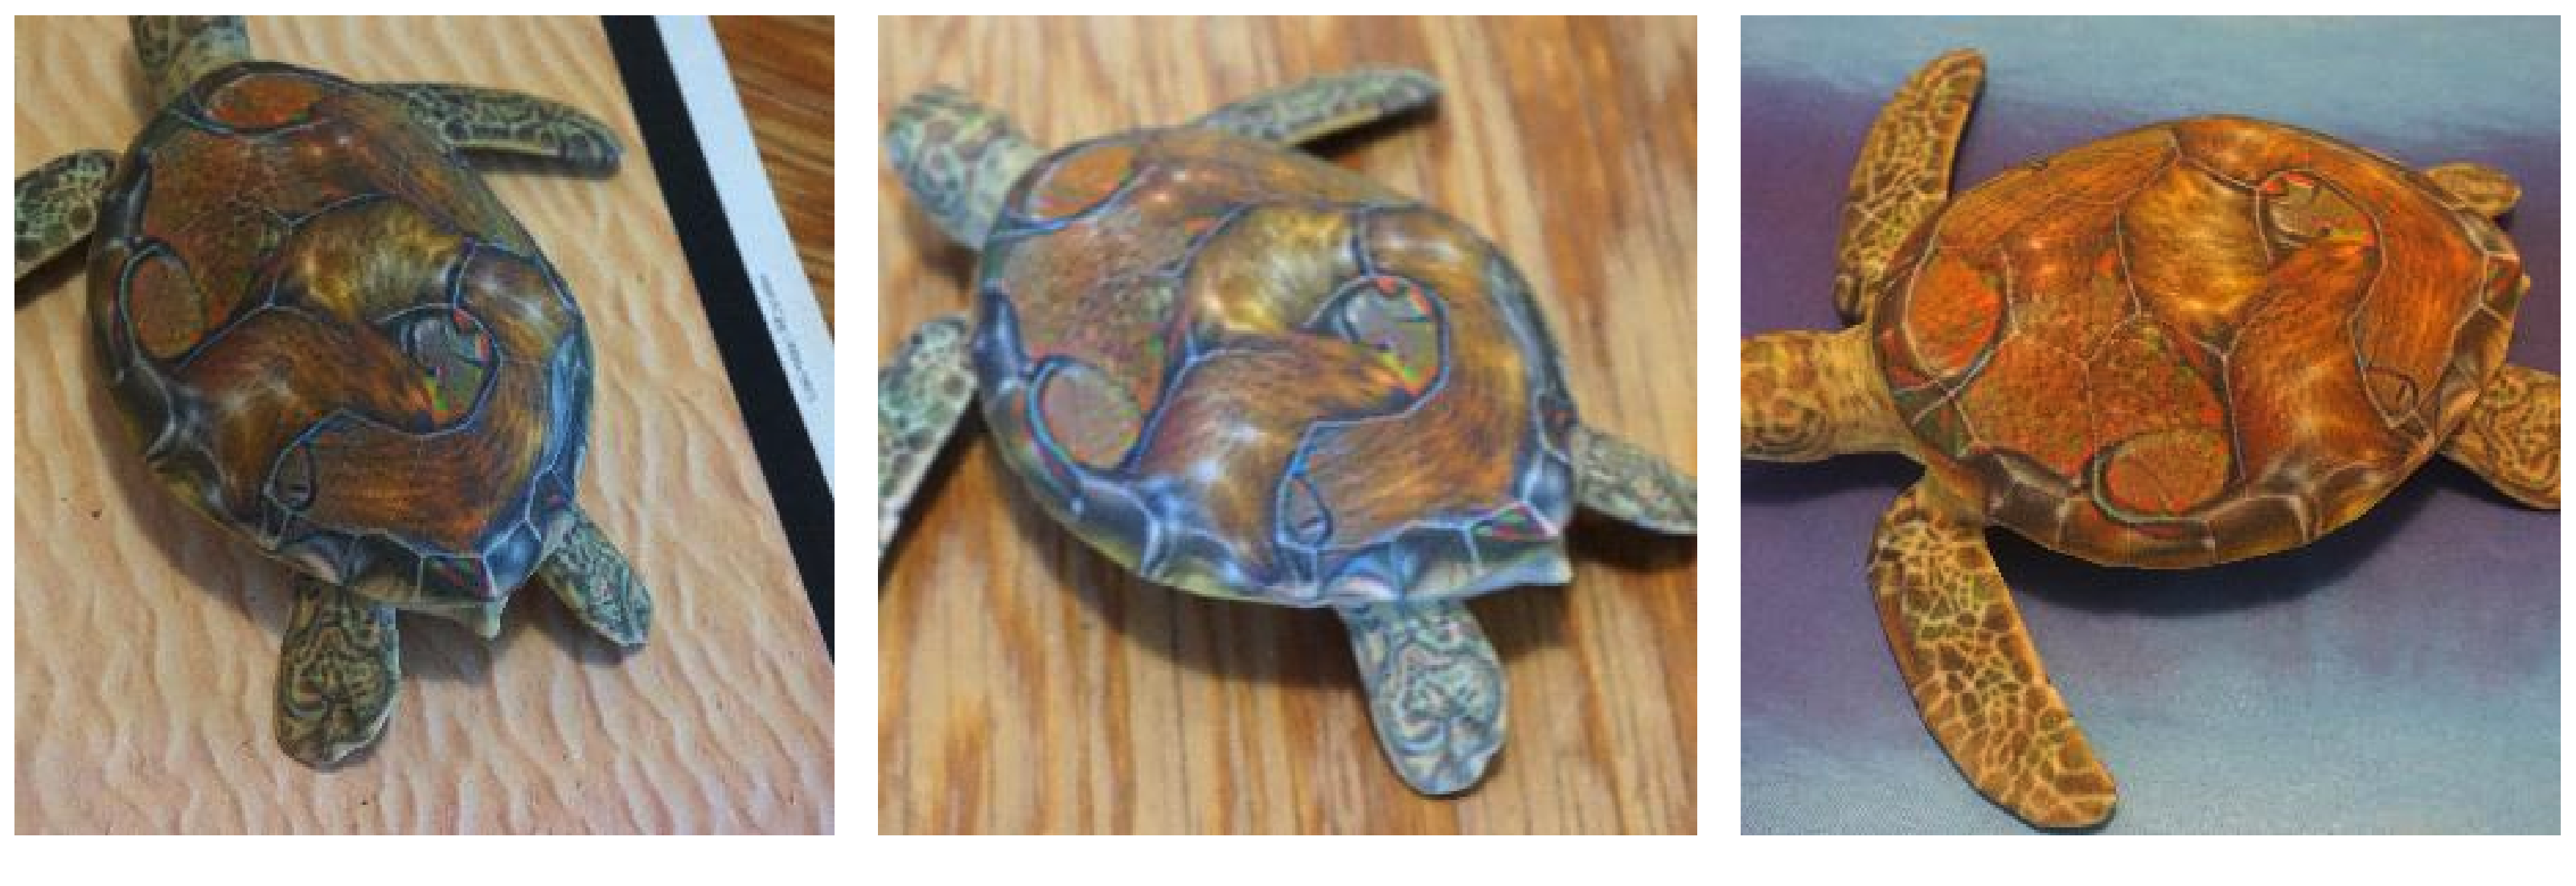
\includegraphics[height=2.7cm]{adversarial_turtle}}\hfill
	\subcaptionbox{Perturbed sign fooling a real car to be read as a 30 speed limit sign. Reproduced from \cite{morgulis2019fooling}\label{fig:adversarialtrafficsign}}{
\includegraphics[height=2.7cm]{adversarial_traffic_sign}}\hfill
	\subcaptionbox{A perturbed logo to be recognised as a \textit{No overtaking} sign. Reproduced from \cite{sitawarin2018darts}\label{fig:adversariallogo}}{
\includegraphics[height=2.7cm]{adversarial_logo}}
	\caption{Many creative approaches for transferring adversarial examples into the physical world have been proposed in academic writing, three of which we are showing here. As machine learning applications experience increasingly widespread adoption in the real world, many researchers warn of points of attack opening up and possibly enabling severe damage.}
	\label{fig:physical}
\end{figure}



Such results matter because robustness is a core requirement for any safety-relevant deployment---which makes it all the more pressing to understand \textit{why} such systems fail, and what that failure implies. It is to those questions that we turn in the following section.

\subsection{Explaining Adversarial Examples}

Having seen \textit{where} adversarial examples arise, we now turn to \textit{why} they exist, highlighting some influential explanation attempts that have been proposed since their discovery in 2013. 

\paragraph{Mysterious Nonlinearity}
The initial paper by Szegedy et al. that introduced the concept of adversarial attacks, already made various core observations that shaped research ever since~\cite{szegedy2013intriguing}. Firstly, they postulated that adversarial examples are neither random artefacts nor isolated anomalies: they occupy entire regions of the input space---\textit{pockets} in the data manifold---that are sparse, and therefore hard to encounter through random sampling, yet can be produced reliably through optimisation. Second, the effect is not merely overfitting. The same adversarial input often fools different models with different hyperparameters, and even different architectures---the phenomenon later called \textit{transferability}---which already argued against attributing adversarial examples to a single model overfitting its training set.

The missing piece that was not offered by their paper was an explanation of the curious phenomenon. Szegedy et al. do postulate that \textit{highly nonlinear model behaviour} might be behind this issue, but no comprehensive explanation was offered. It was only the next year that such explanation attempt was made. 

\paragraph{High-Dimensionality}
The explanation by Goodfellow et al.~\cite{goodfellow2014explaining} can be regarded as one of the most influential in the field. It overturns the intuition, inherited from \cite{szegedy2013intriguing}, that adversarial examples stem from the \textit{extreme non-linearity} of deep networks---highly contorted decision surfaces with rare, low-probability blind spots---possibly compounded by overfitting. Goodfellow et al.\ argued that linear behaviour in high-dimensional spaces is already \textit{sufficient} to produce adversarial examples, refuting the nonlinearity explanation attempt. Because modern networks are often deliberately built to locally behave in near-linear ways (e.g.\ using ReLU) for ease of optimisation, the argument carries over from strictly linear models to deep networks.

The mechanism is a high-dimensional \textit{bloating} effect. For a linear model with weight vector $w$, the response to a perturbed input $x+\eta$---the original input $x$ plus a perturbation $\eta$---is $w^\top(x+\eta) = w^\top x + w^\top\eta$, so the perturbation shifts the activation by $w^\top\eta$. The overall output change of a perturbation thus scales linearly with the number of input dimensions $n$ and mean weight magnitude $m$ with respect to the per-pixel change:
\[
w^\top\eta = \epsilon\sum_{i=1}^{n}\lvert w_i\rvert = \epsilon\, m\, n.
\]
This means that in sufficiently high dimensions, many individually imperceptible, weight-aligned changes accumulate into one large change in the output: the per-pixel budget stays flat as $n$ grows, while the change in the model's output climbs until it crosses the threshold that flips the prediction.

%}.)

The linear view also provided the first explanation of transferability. Since adversarial examples now occupy broad, contiguous half-spaces rather than fine pockets, different models' adversarial regions overlap heavily, which explains why an example crafted for one model tends to fool another at all. And because the discriminative direction is largely a property of the data rather than of the model, models trained on the same task tend to learn similar weight vectors, so that the same perturbation pushes them toward the same incorrect class---which explains why the models tend to agree on that class. 

\paragraph{The Fundamental Mismatch}
Ilyas et al.~\cite{ilyas2019adversarial} shift the framing once more, reframing adversarial examples not as pathological failures but as a \textit{mismatch between machine and human perception}: models exploit patterns that are genuinely predictive, but imperceptible to, and unintuitive for, humans. They distinguish \textit{predictive} features (features correlated with the label) from \textit{robust} features (features that remain predictive under perturbation). Since \textit{empirical risk minimisation} rewards any signal that improves accuracy, a learner will readily rely on predictive but non-robust features; adversarial vulnerability is then an expected consequence of standard training, rooted in the gap between the human sense of similarity and the statistical structure of the data. A striking experiment makes this concrete: they relabel every image of CIFAR-10 with a new, random target class and perturb it so that a model reads the new label, while to a human the images appear unchanged and hence entirely mislabelled. A standard model trained on this dataset nevertheless generalises well to the \textit{clean}, unmodified test set---evidence that it has latched onto real, transferable features that merely happen to be imperceptible to us. This view also bears on interpretability: if a model succeeds by relying on human-imperceptible features, there may be little in its decisions for a human to understand.

\begin{figure}[t]
    \centering
    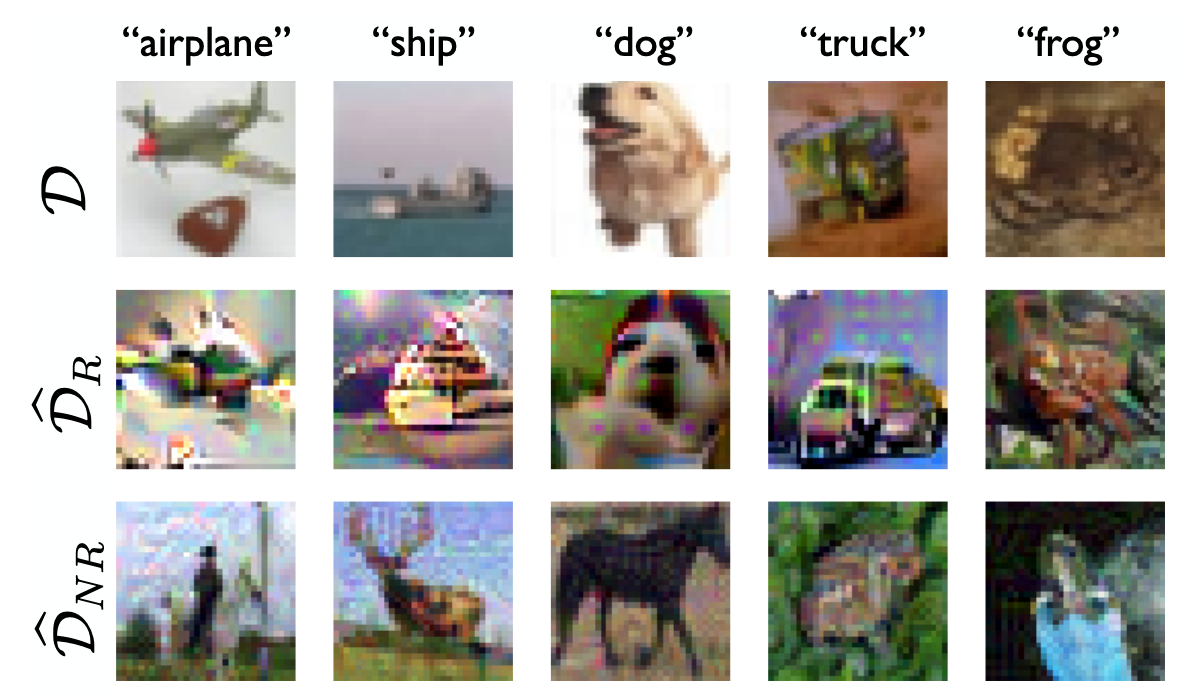
\includegraphics[height=3.5cm]{adversarial_dataset}
    \caption{Ilyas et al.'s feature experiment~\cite{ilyas2019adversarial}. \emph{Top:} original CIFAR-10 images. \emph{Middle:} the extracted predictive but non-robust features---barely recognisable to a human, yet highly informative to a model. \emph{Bottom:} the resulting set of (relabelled) adversarial examples, which looks entirely mislabelled to a human but still trains a classifier that generalises correctly to the clean test set.}
    \label{fig:explaining}
\end{figure}


\subsection{Pertinence of Adversarial Examples as a Subject Area}

The two preceding subsections shed an interesting light on adversarial attacks as a field of study in the domain of cyber security. In the first, we asked whether they pose a real danger and found that little evidence can be found that adversarial attacks pose a pertinent security threat in any practical scenario. As a live security threat they have so far been marginal, dwarfed by cruder and cheaper forms of attack~\cite{apruzzese2023real, raff2023dont}. Adding in our examination of different explanations for the phenomenon, we come to the conclusion that the primary significance of adversarial examples is of \textit{epistemic} nature. Their main impact can be seen as offering a new view on the inherent vulnerabilities of machine learning systems; shaking up pre-existing beliefs. In other words, their importance lies less in what they let an attacker do than in what they reveal about the systems they target.

What they reveal is considerable. Before the discovery and systematic study of adversarial examples, machine-learning models were evaluated almost exclusively on accuracy, and robustness was expected only implicitly~\cite{biggio2018wild, hendrycks2019benchmarking}. Adversarial examples showed that high test accuracy does not imply that a model has grasped a learning task the way a human would: a classifier will confidently mislabel an input that is, to a human observer, semantically unchanged. This was the original observation that made the phenomenon of adversarial attacks so remarkable. This forced a more intricate account of how machine learners operate---from Goodfellow et al.'s high-dimensional linearity to Ilyas et al.'s reframing of adversarial features as genuine but human-imperceptible signal~\cite{goodfellow2014explaining, ilyas2019adversarial}---and, with it, a redefinition of \textit{robustness} from an assumed by-product of accuracy into a distinct property that must be explicitly demanded, engineered, and evaluated. This shift is not merely academic: as machine learning is embedded in autonomous vehicles, border control, and surveillance, physical adversarial attacks make plain that robustness cannot be taken for granted in exactly those deployments where its absence would be most costly.

Viewed from a distance, the lesson generalises well beyond the field. When we trust a simple mathematical proxy to stand in for a messy real-world objective---as an overriding focus on accuracy does for machine learners---we are bound to be disappointed, and the resulting mismatch can surface suddenly and in unexpected ways. The contribution of adversarial examples is to have made that mismatch---between human and machine notions of similarity and understanding---impossible to ignore.

\section{Conclusion}

This report has given a broad overview of adversarial attacks in machine learning. After defining adversarial examples and organising the field along a clear taxonomy, we surveyed the most influential methods. We then stepped back to consider adversarial attacks in the real and physical world, the competing attempts to explain why they exist, and what their study has contributed to the field.

Our central conclusion is that the significance of adversarial examples is primarily \textit{epistemic}. As a practical security threat they have so far been marginal, their lasting impact lies in what they reveal about machine learning itself. They demonstrated that high test accuracy does not mean a human-like grasp of a task, exposed a fundamental mismatch between human and machine perception, and turned \textit{robustness} from an implicit assumption into a property that must be explicitly defined, demanded, and asserted.

\section*{Statement of Contributions}

Bjarne Thal: Introduction (1), Definition of adversarial examples (2.1), Taxonomy (2.2), L-BFGS, DeepFool, Carlini-Wagner, Discussion (3), Conclusion (4)

Marius Wrobel: FGSM, Variants of FGSM, PGD, Transfer Attacks (Jacobian-based, Ensemble Attacks, Momentum), ZOO, Notable Poisoning Attacks (2.4)

Both of us conducted literature search.

\printbibliography

\newpage
\pagestyle{empty}

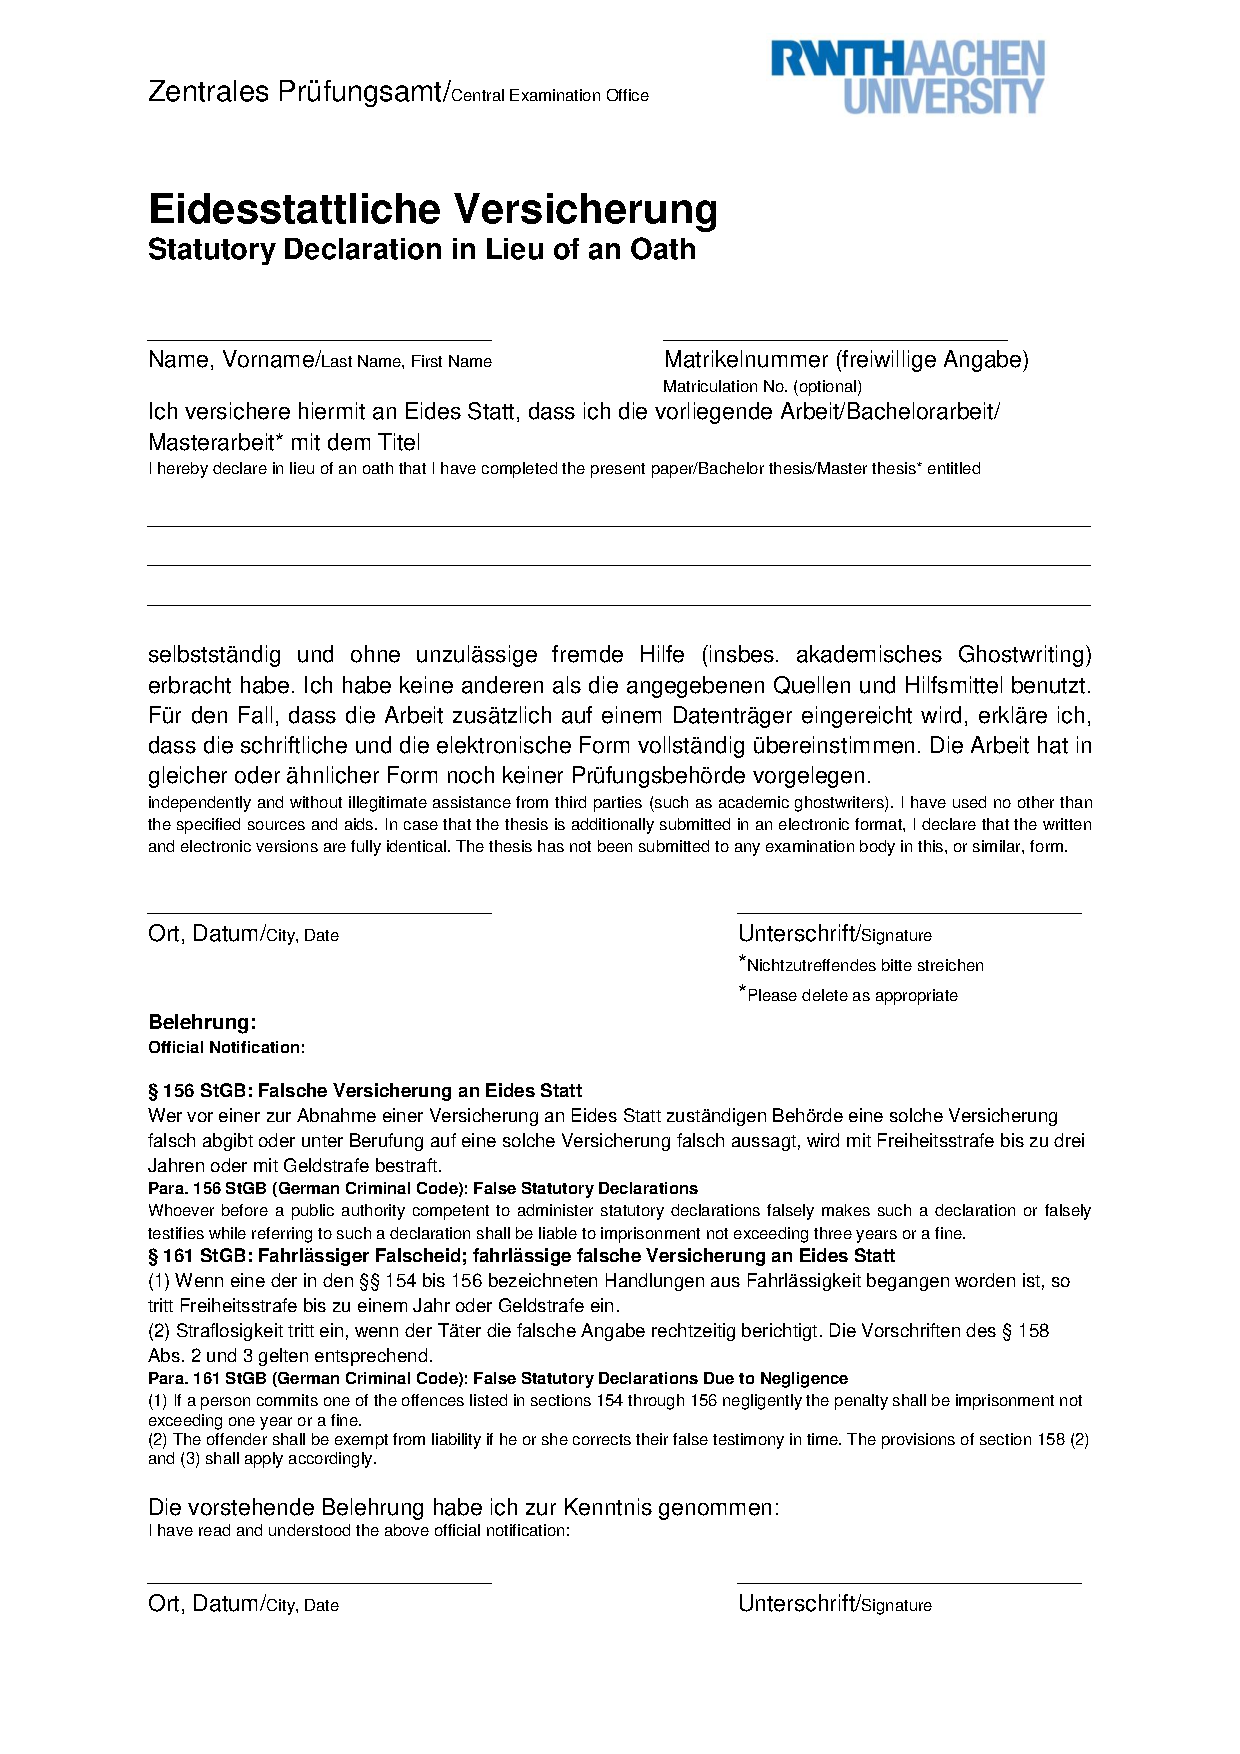
\includepdf[pages=-,pagecommand={},width=\textwidth]{files/oathstatement.pdf}

\end{document}
